\section{Experiments}
\label{sec:exp}
	To illustrate the potential of the theoretical model presented in section \ref{sec:method}, we implemented an example to analyze the practical aspect as well as the empirical results.

In this section, we will proceed to describe our experimental settings, explain choices related to the implementation, and present the resulting data as well as the conclusions we draw from them.

\subsection{Code-level optimizations}

A group of code-level optimizations have been identified and compiled by previous work \cite{engstrom2020implementation}\cite{shengyi2022the37implementation} in an effort to reproduce reported results for the PPO algorithm. 

It is worth  noting that while none of these optimizations are formally included in the basic definition of the algorithm or credited for its performance, some of them are a de-facto part of any functional implementation, especially those that relate to compatibility with  continuous space environments. The rest are not strictly required for the algorithm to function. Nonetheless, they are needed to reproduce the state-of-the-art results and are, as a rule, included in benchmark implementations \cite{huang2021cleanrl} \cite{baselines}.

Due to the ill-defined nature of what constitutes a baseline for PPO or what degree of optimization still falls within the scope of the algorithm, we have elected to implement and run a minimalist interpretation of the algorithm with only enough optimizations to be functional and to support the environments we test on. We used the Keras library to implement the neural networks and their optimizations.

This implementation does not therefore reproduce the highest reported results for PPO. Instead, we report improvement from our method only in relation to our own implemented baseline, as the purpose of this research is to establish the effect of our contribution by comparison to a similar basis that does not implement it.

Following are the optimizations and the main reason for their inclusion:

\begin{description}
\item[Support for continuous action space environments] %(mean and std as output instead of logits(??))
 We modify the policy network to make it output both the mean and the standard deviation in order to sample actions from a gaussian distribution, instead of a categorical distribution in the case of environments with discrete action spaces.
 
\item[Advantage normalization] while this optimization does not necessarily improve the final performance\cite{andrychowicz2020learning}, it helps greatly in stabilizing the training process.
%Advantage norm essentially doesn't make your gradients go insane, and you also get an equal number of positive gradients to negative gradients, making your policy weights not go insane (which is why you tend to see more stable training) But at the tail end of training, if your algo is stable 'enough', the gradients at the end of training are really miniscule anyway, and do nothing to improve final performance
\item[Reward scaling] We divide the rewards by the (estimated) standard deviation of the discounted cumulative rewards at step $t$ by a factor $\gamma$: $R_t = \sum_{i=0}^t \gamma^{t-i} r_i$. %This optimization was only used for training on the Hopper task.
\item[KL fallback] Approximates the Kullback-Leibler (KL) divergence and cancels a policy update if the value is above a threshold. Implemented to prevent catastrophic unlearning\cite{dossa2021empirical}, a phenomenon observed in PPO where a suboptimal update causes the average episodic reward to drop brusquely and never recover.
\end{description}

\subsection{Testing Setup}

Our experiment setting consists of four robotic tasks from the Pybullet suite of environments using Gym. Gym\cite{brockman2016openai} is an open source toolkit for RL research initially released by OpenAI. 

We run the algorithm on the four continuous tasks with different settings (baseline PPO, PPO with Generalized Critic, PPO with Generalized Critic + bootstrap). We run each configuration over 10 random seeds and track the recorded returns using Weights and Biases\cite{wandb}.

For each of the critics, we estimate the advantage function using the Generalized Advantage Estimation method\cite{schulman2015highdimensional}.
The hyperparameters are detailed in table %\ref{hyperparameters}

\begin{table}
  \begin{center}
    \begin{tabular}{cc}
      \hline 
      hyperparameter & value \\ 
      \hline 
      \verb!total timesteps! & \verb!2M! \\
      \verb!PPO update iterations per epoch! &  \verb!80! \\
      \verb!GAE gamma! & \verb!0.99! \\
      \verb!GAE lambda! & \verb!0.97! \\
      \verb!kl_target! & \verb!0.1! \\
      \verb!(policy network) hidden layers! & \verb![120, 84]! \\
      \verb!(policy network) learning_rate! & \verb!3e-4! \\
      \verb!(policy network) activation function! & \verb!relu!\\
      \verb!(value network) hidden layers! & \verb![64]! \\
      \verb!(value network) learning_rate! & \verb!3e-4! \\
      \verb!(value network) activation function! & \verb!relu! \\
      \hline      
    \end{tabular}
  \end{center}
  \caption{Experiment hyperparameters and their values}
  \label{hyperparameters}
\end{table}




%\subsection{Experiment tracking}
 



%Good for Hopper
% Meh for Humanoid
% bad for hc? smth bl3t

\subsection{Experimental Results and Analysis}

We notice that changes in performance depend highly on the testing environment. 
As in figure \ref{exp2}, Hopper is the most reliably improved, followed by Humanoid.

GC (without bootstrap) tends to improve on minimal values, which may indicate a reduction in the number of non-converging runs.

GC (with bootstrap) reaches better performance across environments, potentially indicating that multiple critics/value function estimates help reach better optimization goals in the same amount of runs, which would make it more sample-efficient.

%analysis
% comment the figures

\begin{table}
  \begin{center}
\begin{tabular}{p{0.35\textwidth}|p{0.2\textwidth}p{0.2\textwidth}p{0.2\textwidth}}
    \hline
    & Baseline PPO & GC with bootstrap & GC without bootstrap \\
    \hline
    Inverted Double Pendulum & (\textbf{1530.122}, 7197.542) & (1458.429, \textbf{9358.719}) & (1227.872, 9358.412) \\
    \hline
    Half Cheetah & (-1487.176, \textbf{484.245}) & (-1033.386, 411.735) & (\textbf{-970.766}, 465.321)\\
    \hline
    Hopper & (646.152, 901.31) & (748.151, 899.803) & \textbf{(754.571, 908.167)} \\
    \hline
    Walker 2D & (95.908, 427.7) & (86.125, \textbf{656.49}) & (\textbf{204.608}, 593.467) \\
    \hline  
\end{tabular}
  \end{center}
  \caption{Final performance for each training set (min, max)}
  \label{hyperparameters}
\end{table}

Different configurations converge better with different random seeds (see figure \ref{seeds})


\begin{figure}[!htb]
\begin{minipage}[b]{.5\linewidth}
  \centering
  \centerline{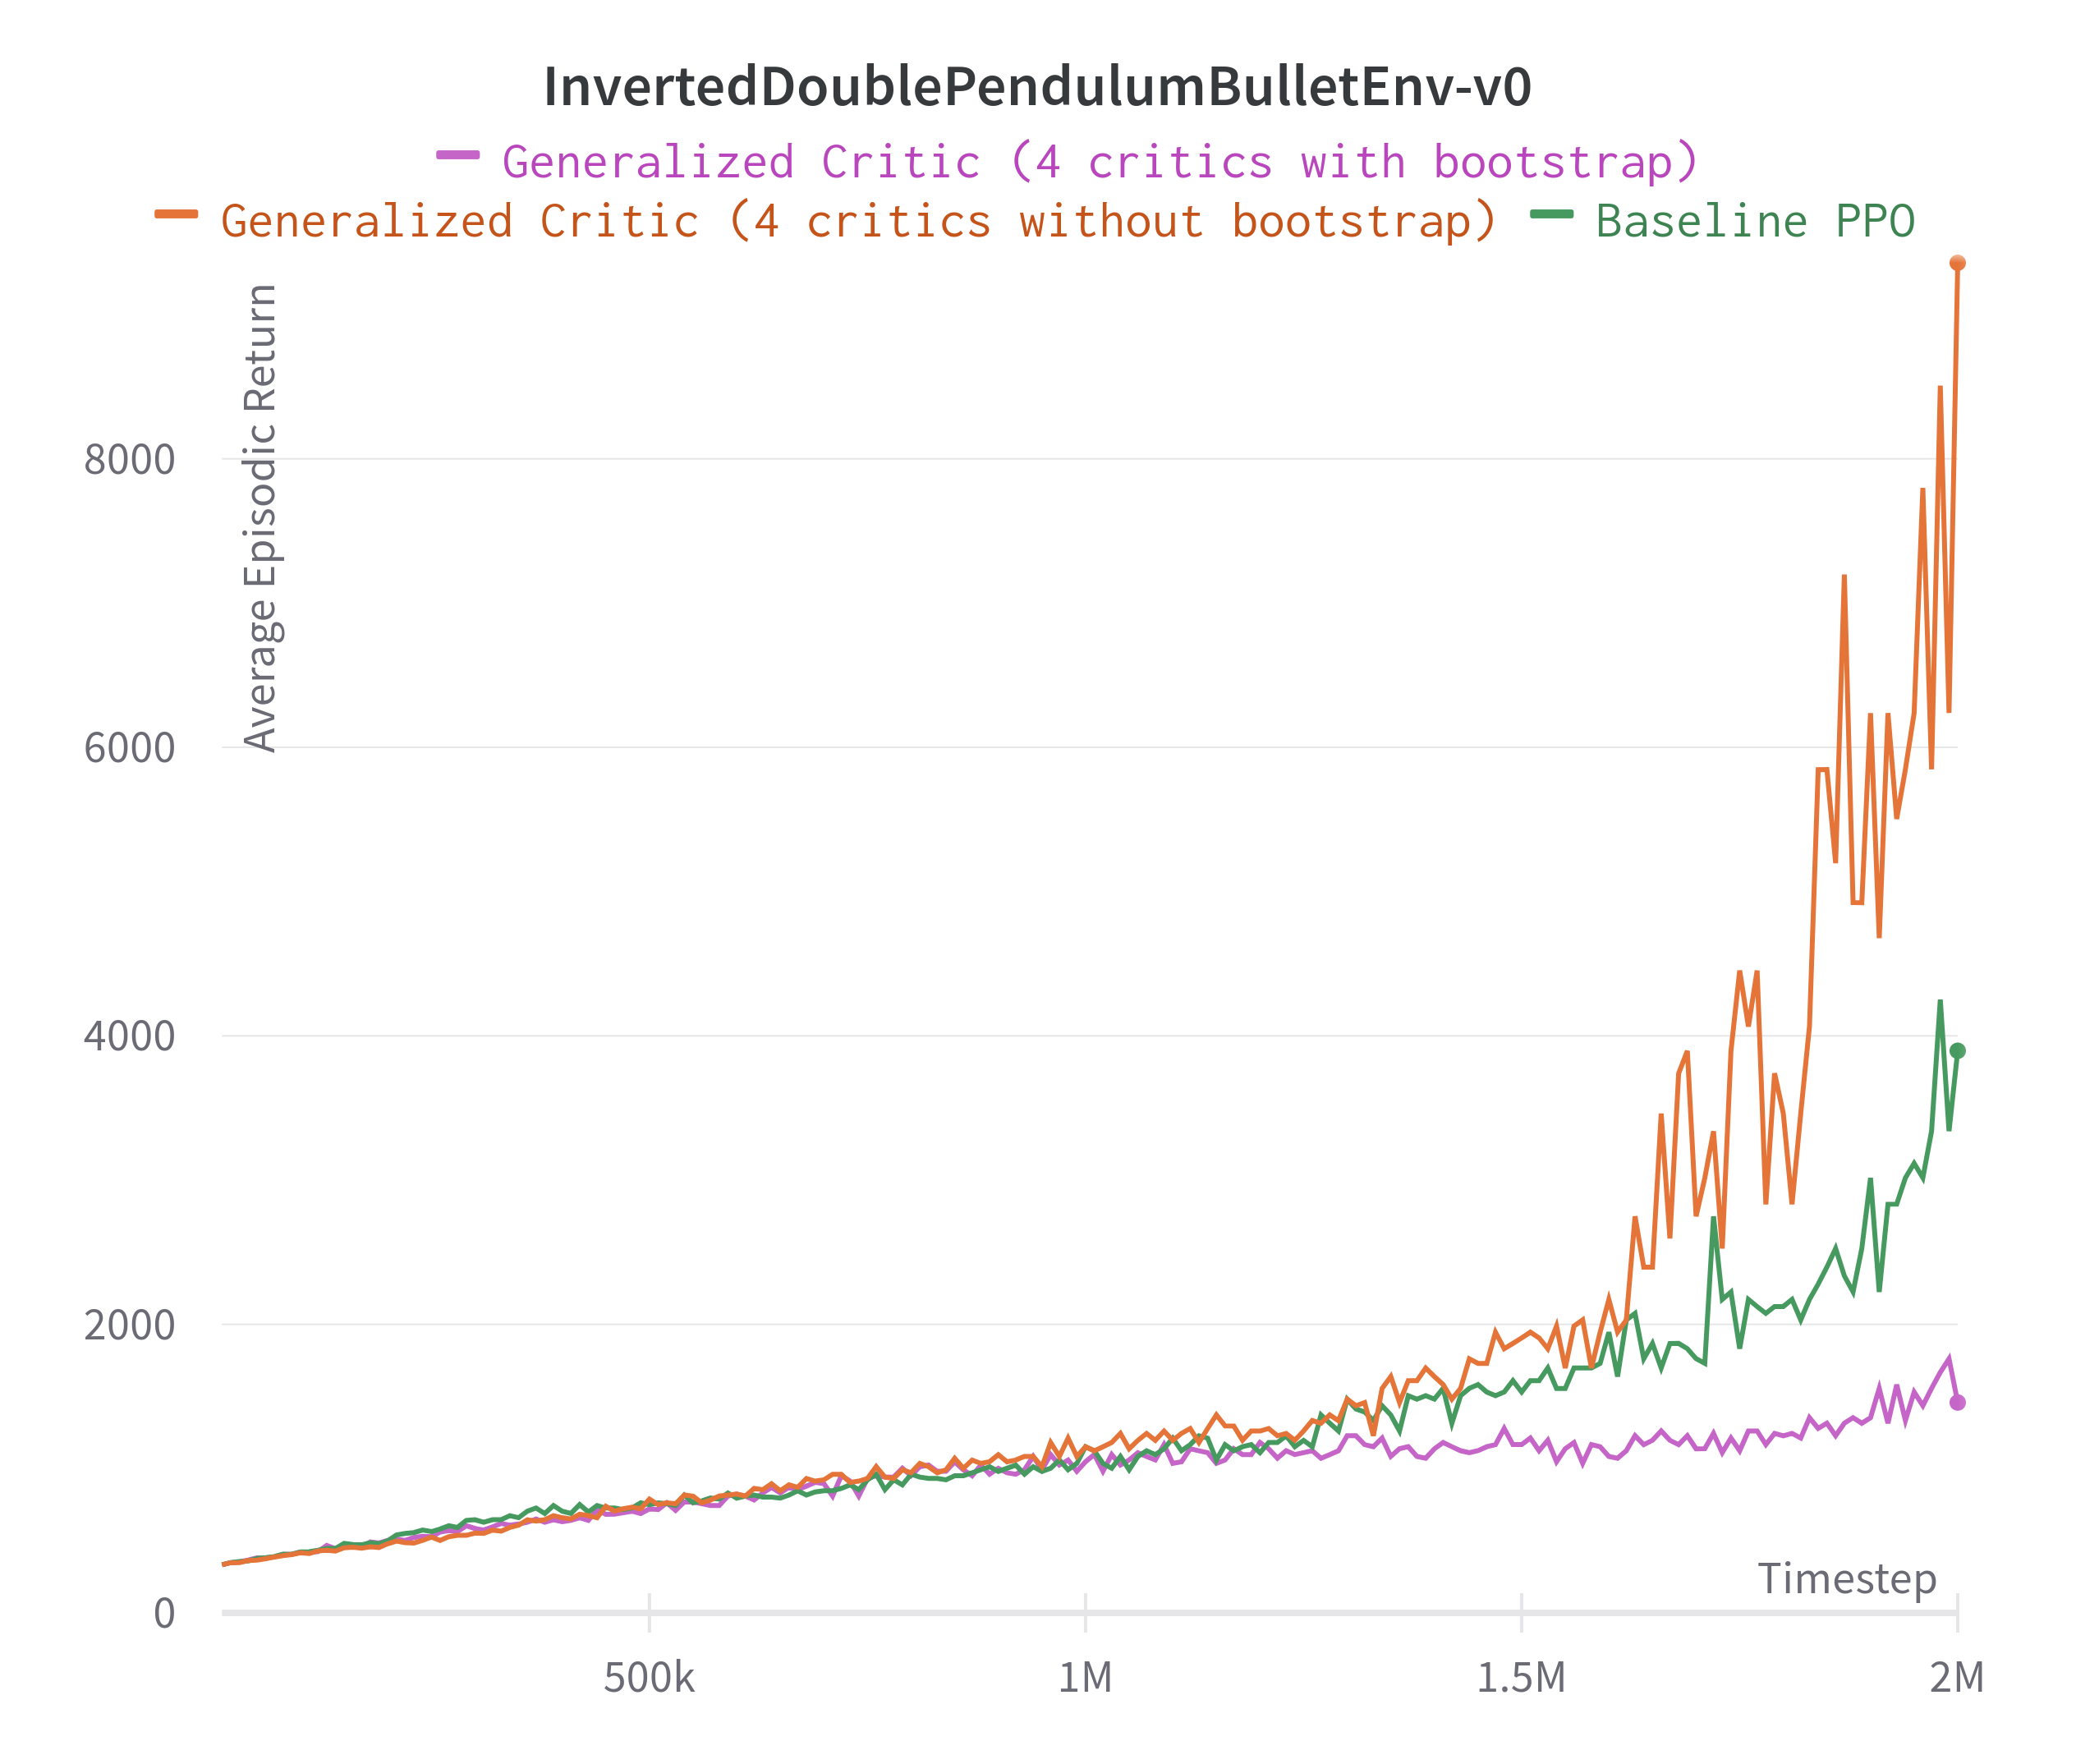
\includegraphics[width=\linewidth]{images/idpseed90}}
%  \vspace{2.0cm}
%  \centerline{(a) Walker2DBulletEnv-v0}\medskip
\end{minipage}
\begin{minipage}[b]{.5\linewidth}
  \centering
  \centerline{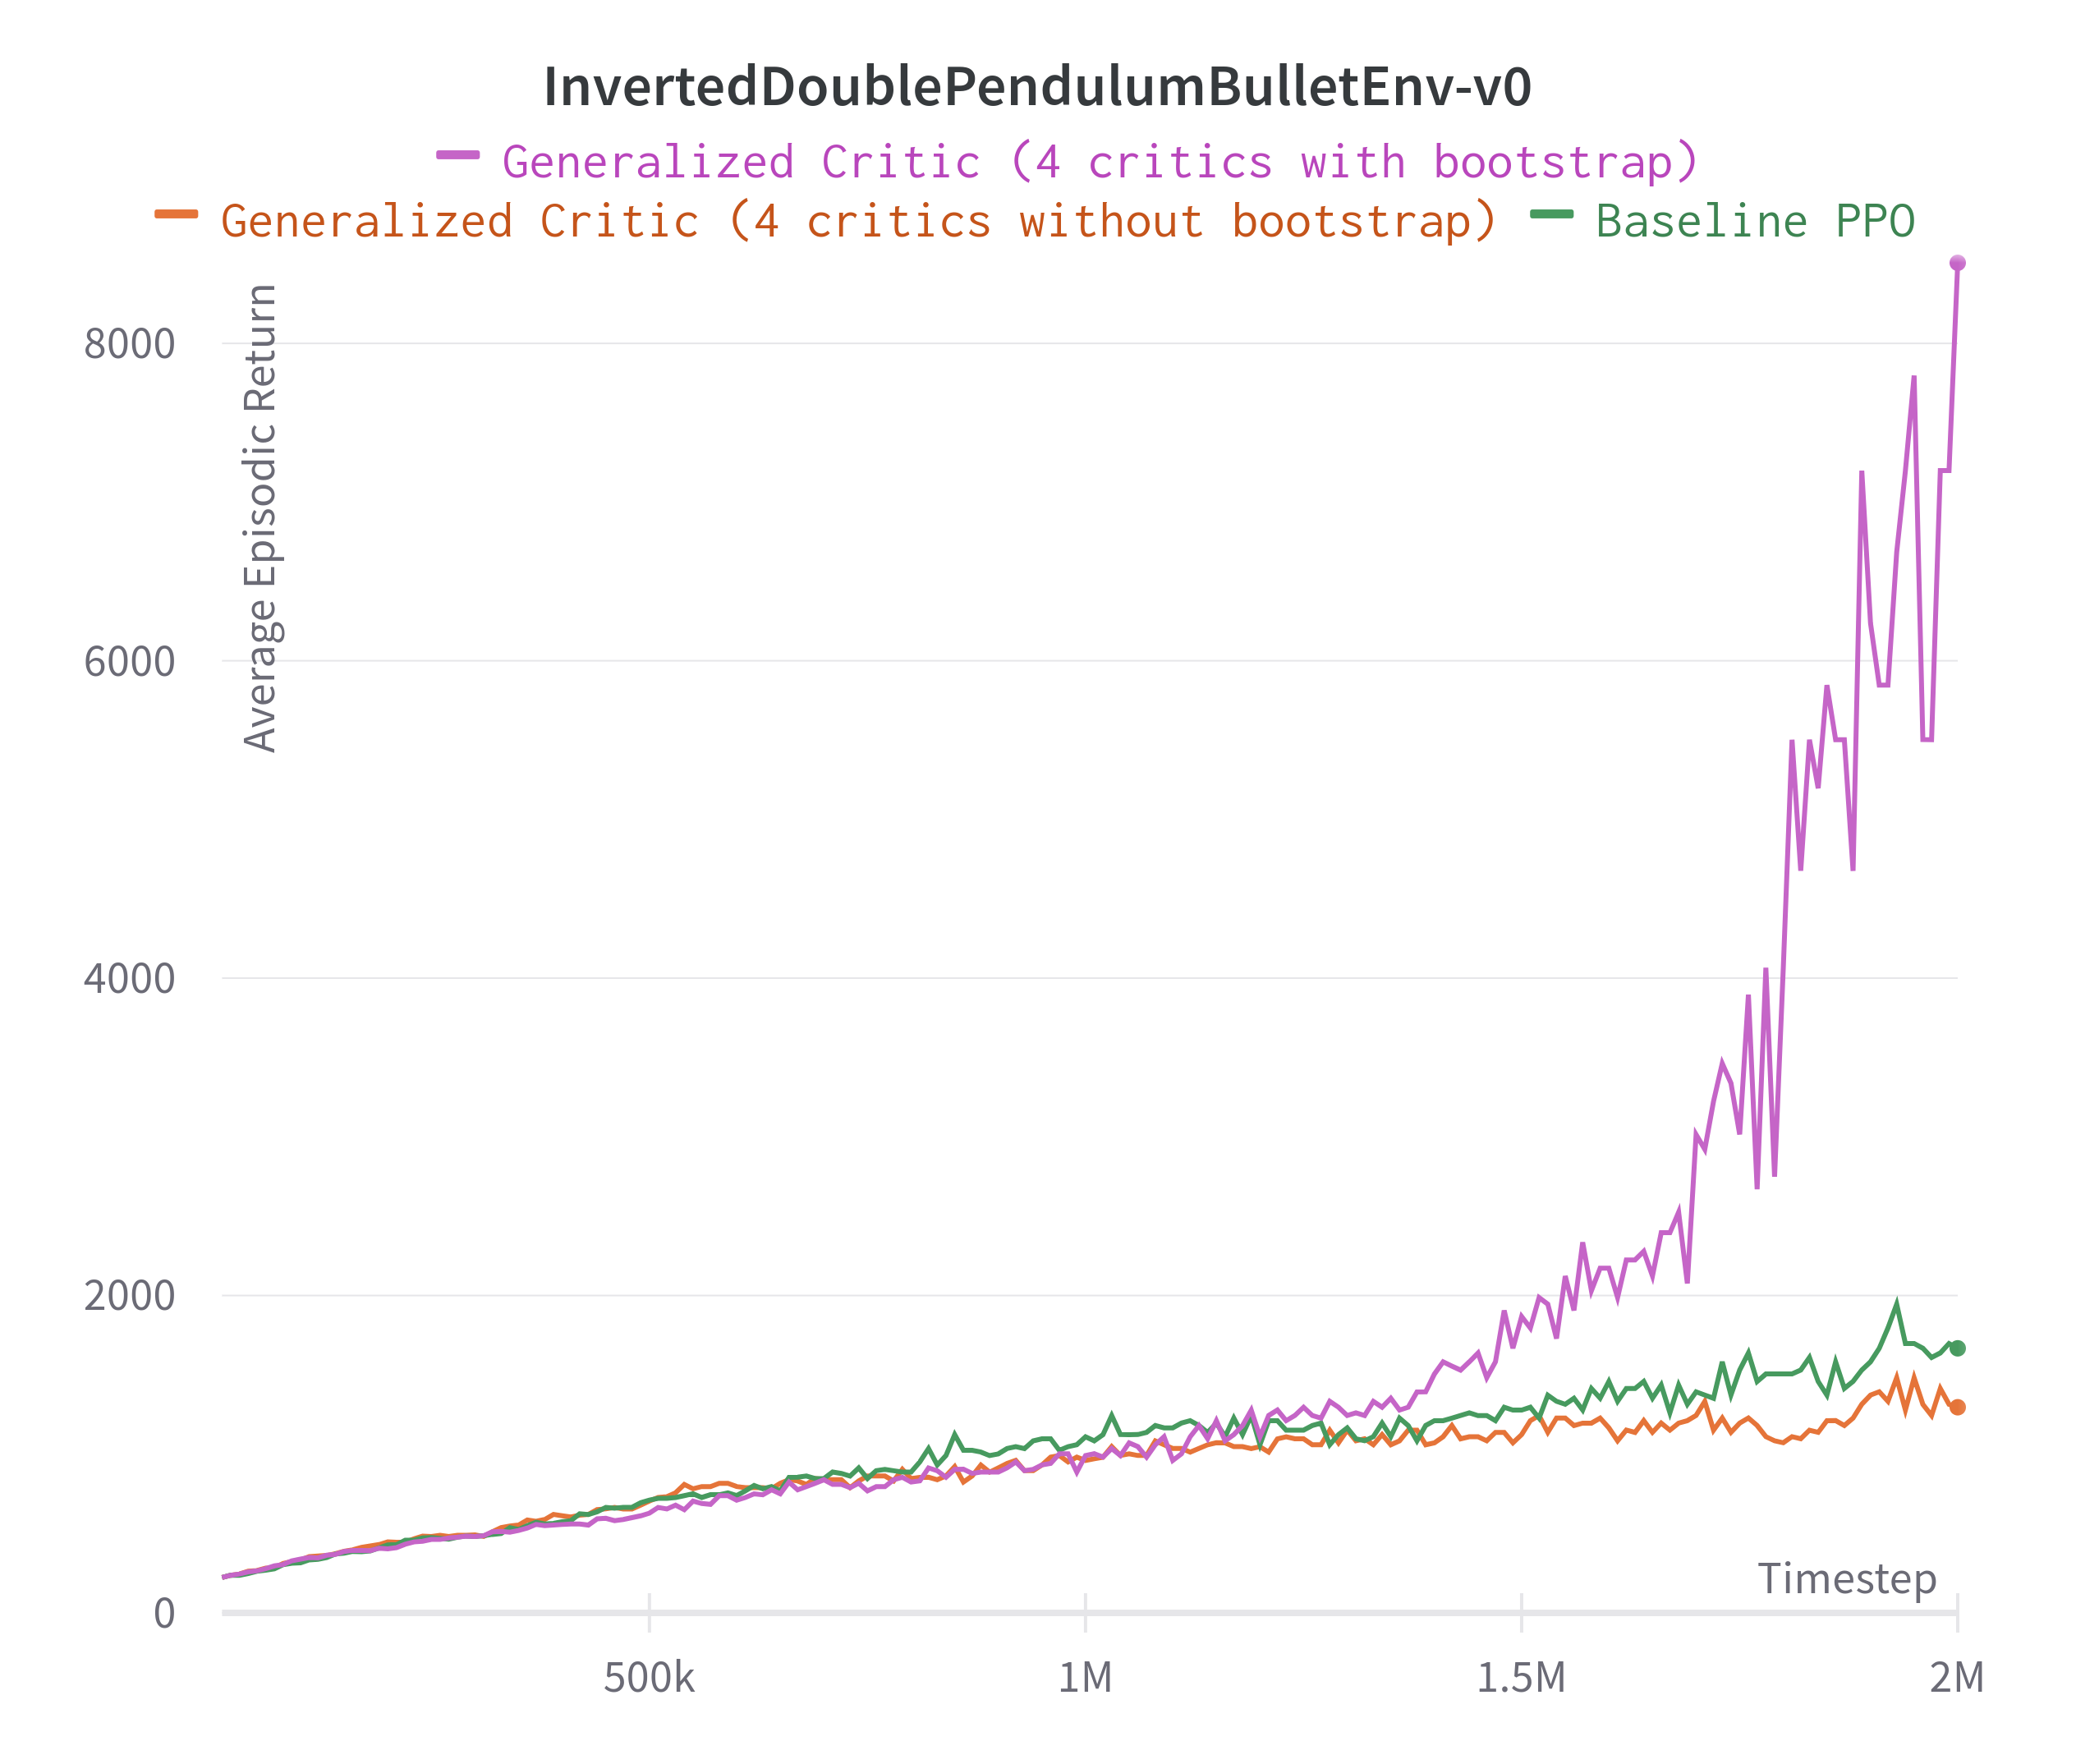
\includegraphics[width=\linewidth]{images/idpseed80}}
%  \vspace{2.0cm}
%  \centerline{(b) HalfCheetahBulletEnv-v0}\medskip
\end{minipage}
  \caption{Two identical runs of InvertedDoublePendulumBulletEnv with different random seeds}
  \label{seeds}
\end{figure}

\begin{figure}[!htb]
\begin{minipage}[b]{.5\linewidth}
  \centering
  \centerline{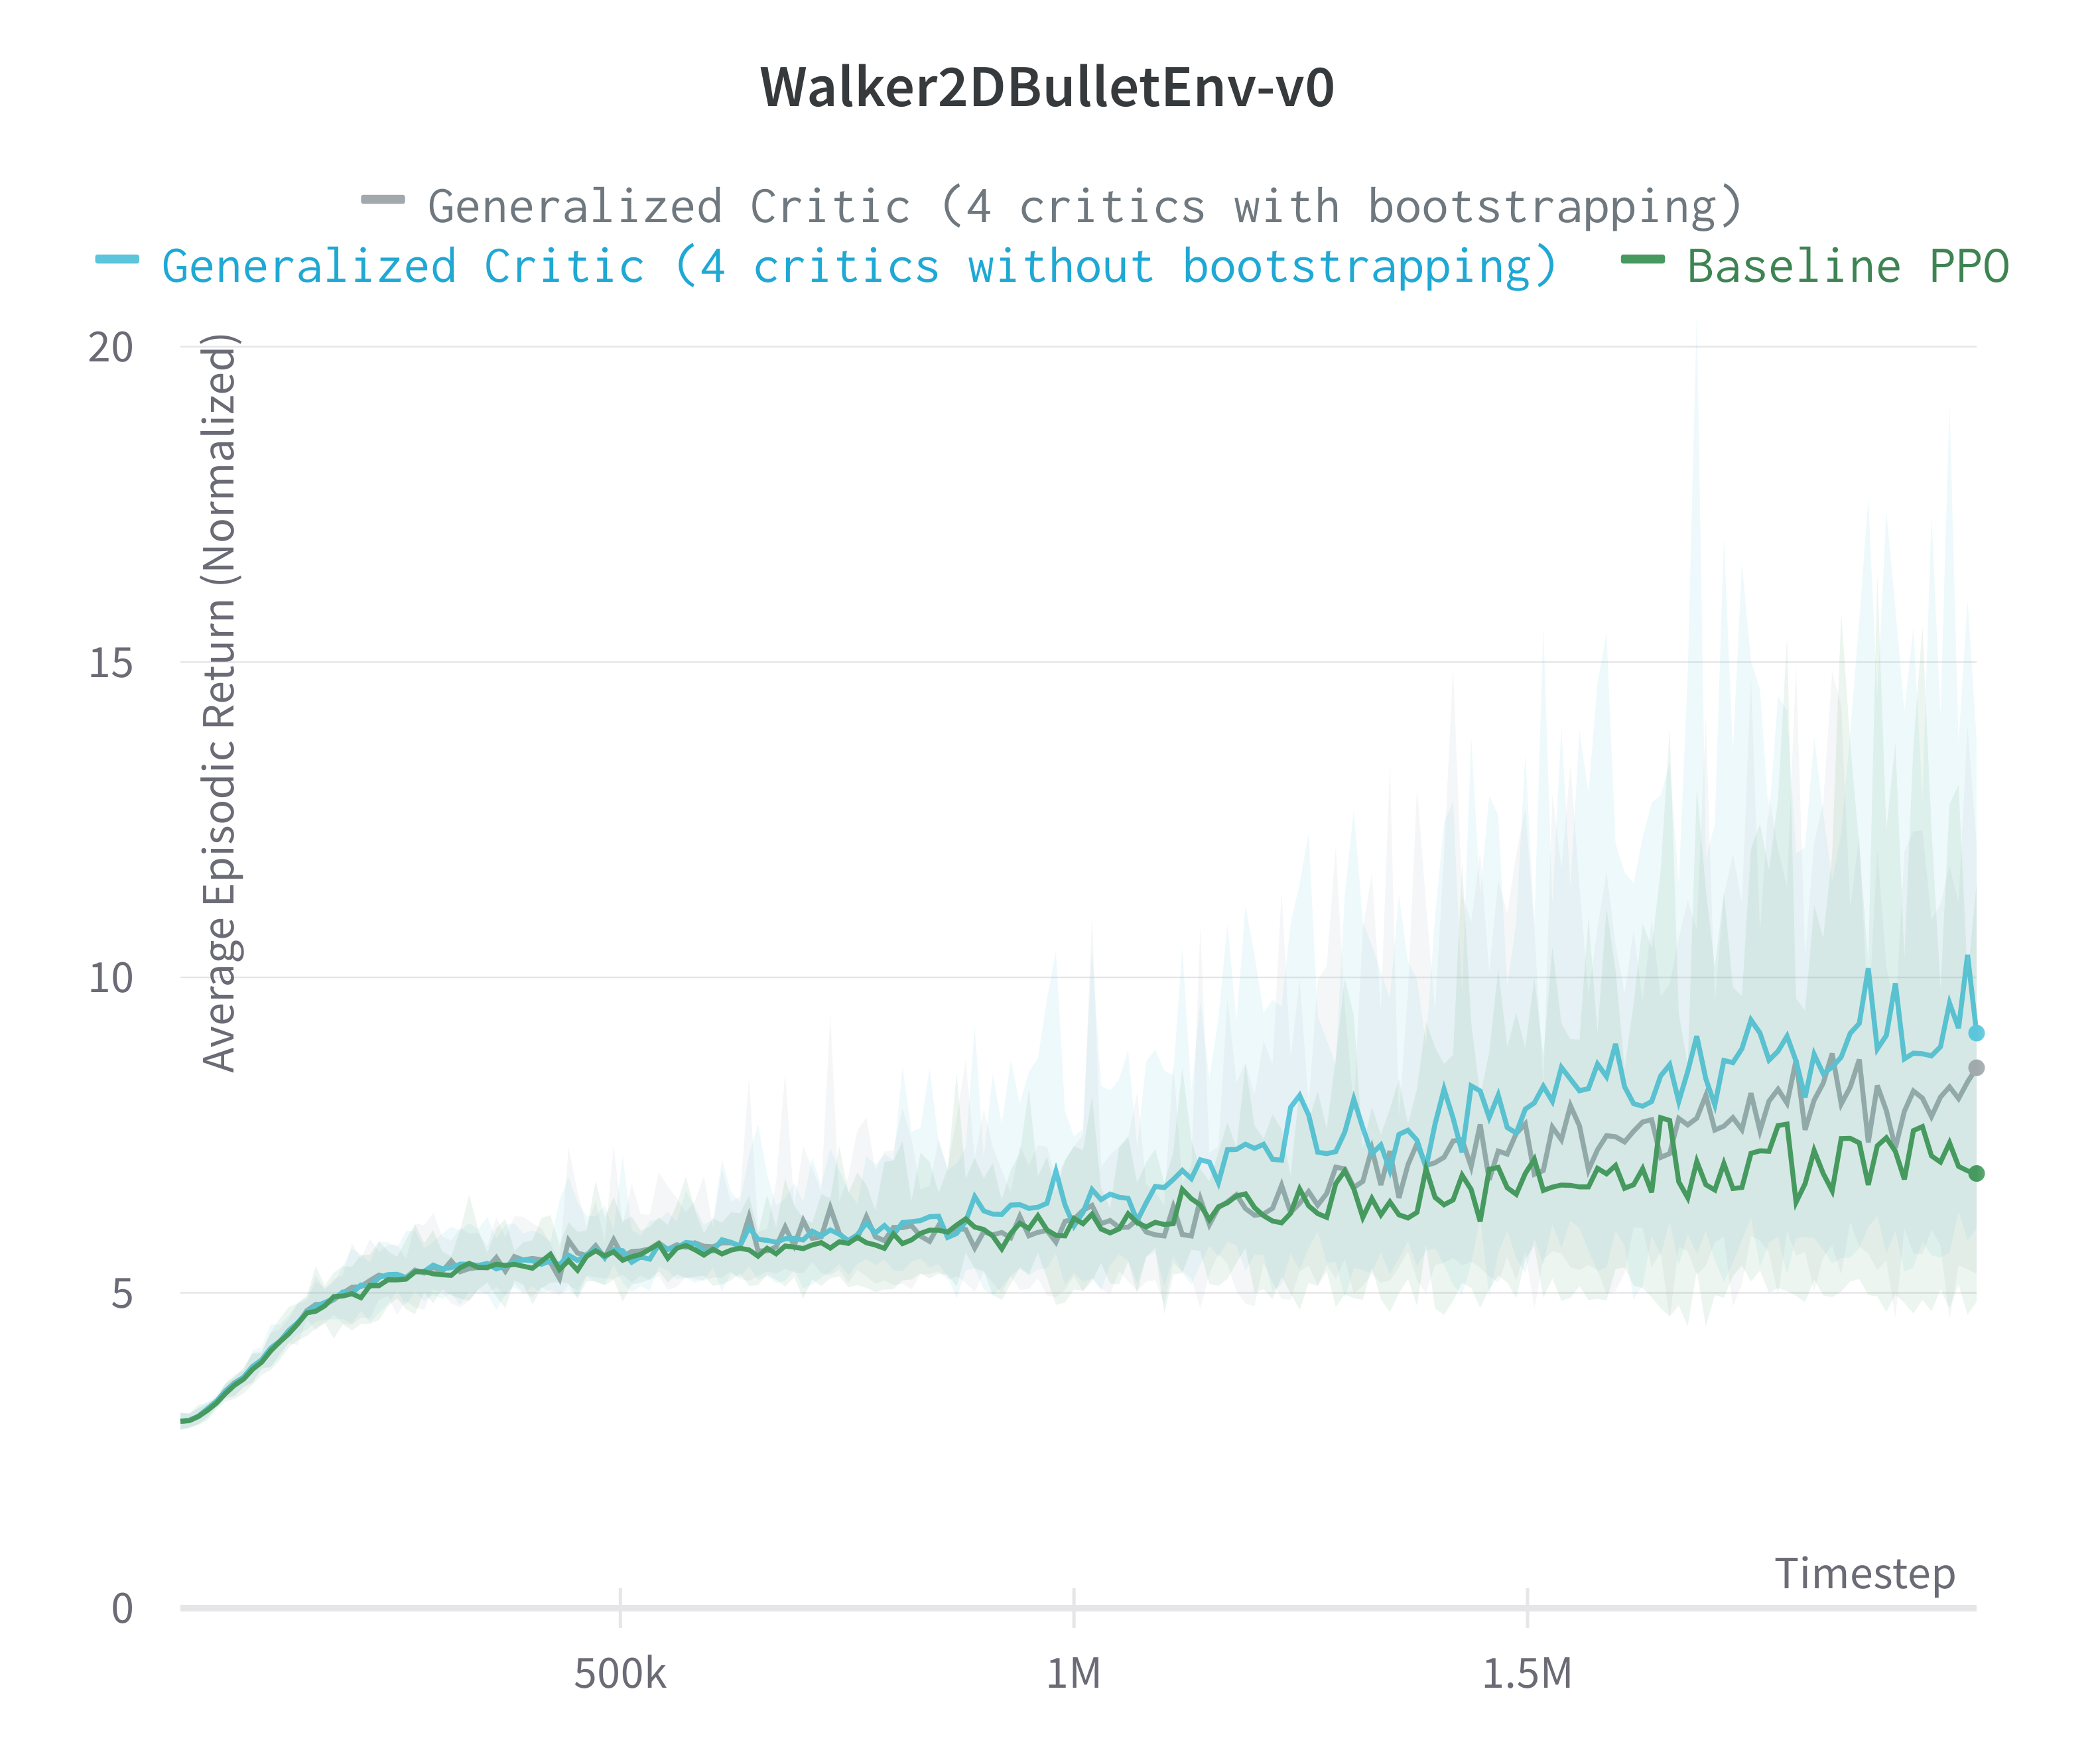
\includegraphics[width=\linewidth]{images/walker2D}}
%  \vspace{2.0cm}
%  \centerline{(a) Walker2DBulletEnv-v0}\medskip
\end{minipage}
\begin{minipage}[b]{.5\linewidth}
  \centering
  \centerline{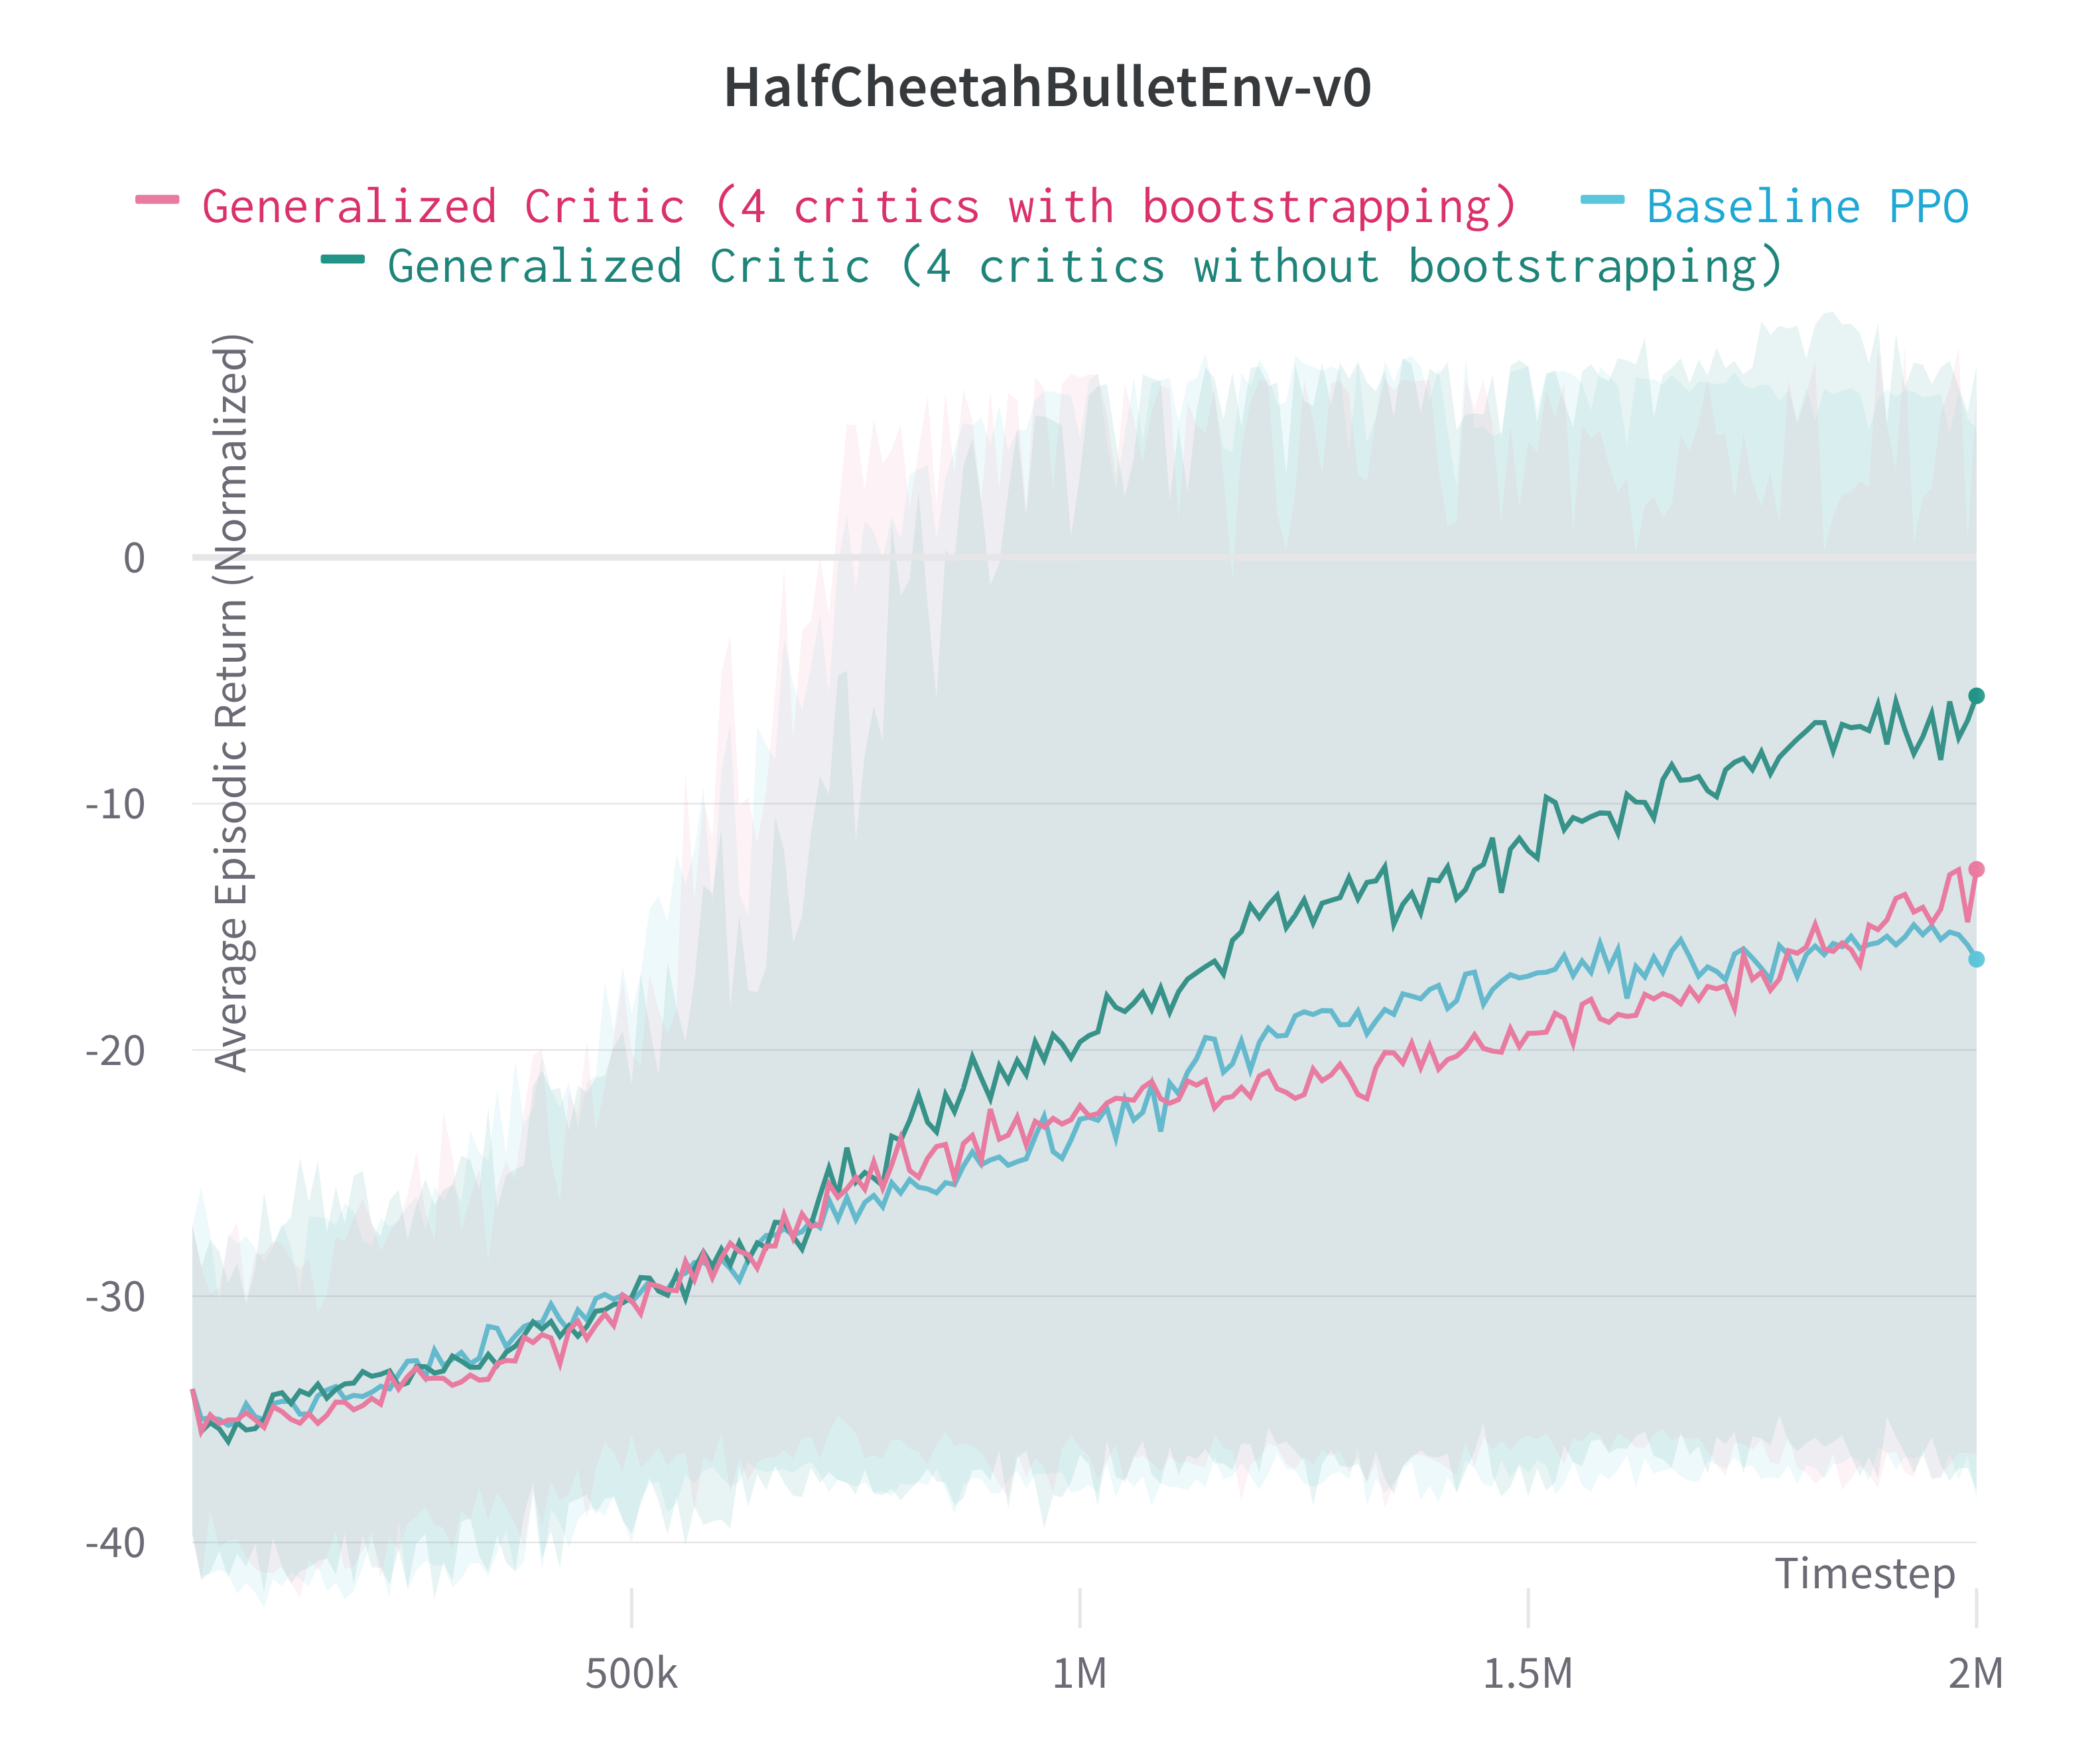
\includegraphics[width=\linewidth]{images/halfcheetah}}
%  \vspace{2.0cm}
%  \centerline{(b) HalfCheetahBulletEnv-v0}\medskip
\end{minipage}

\begin{minipage}[b]{.5\linewidth}
  \centering
  \centerline{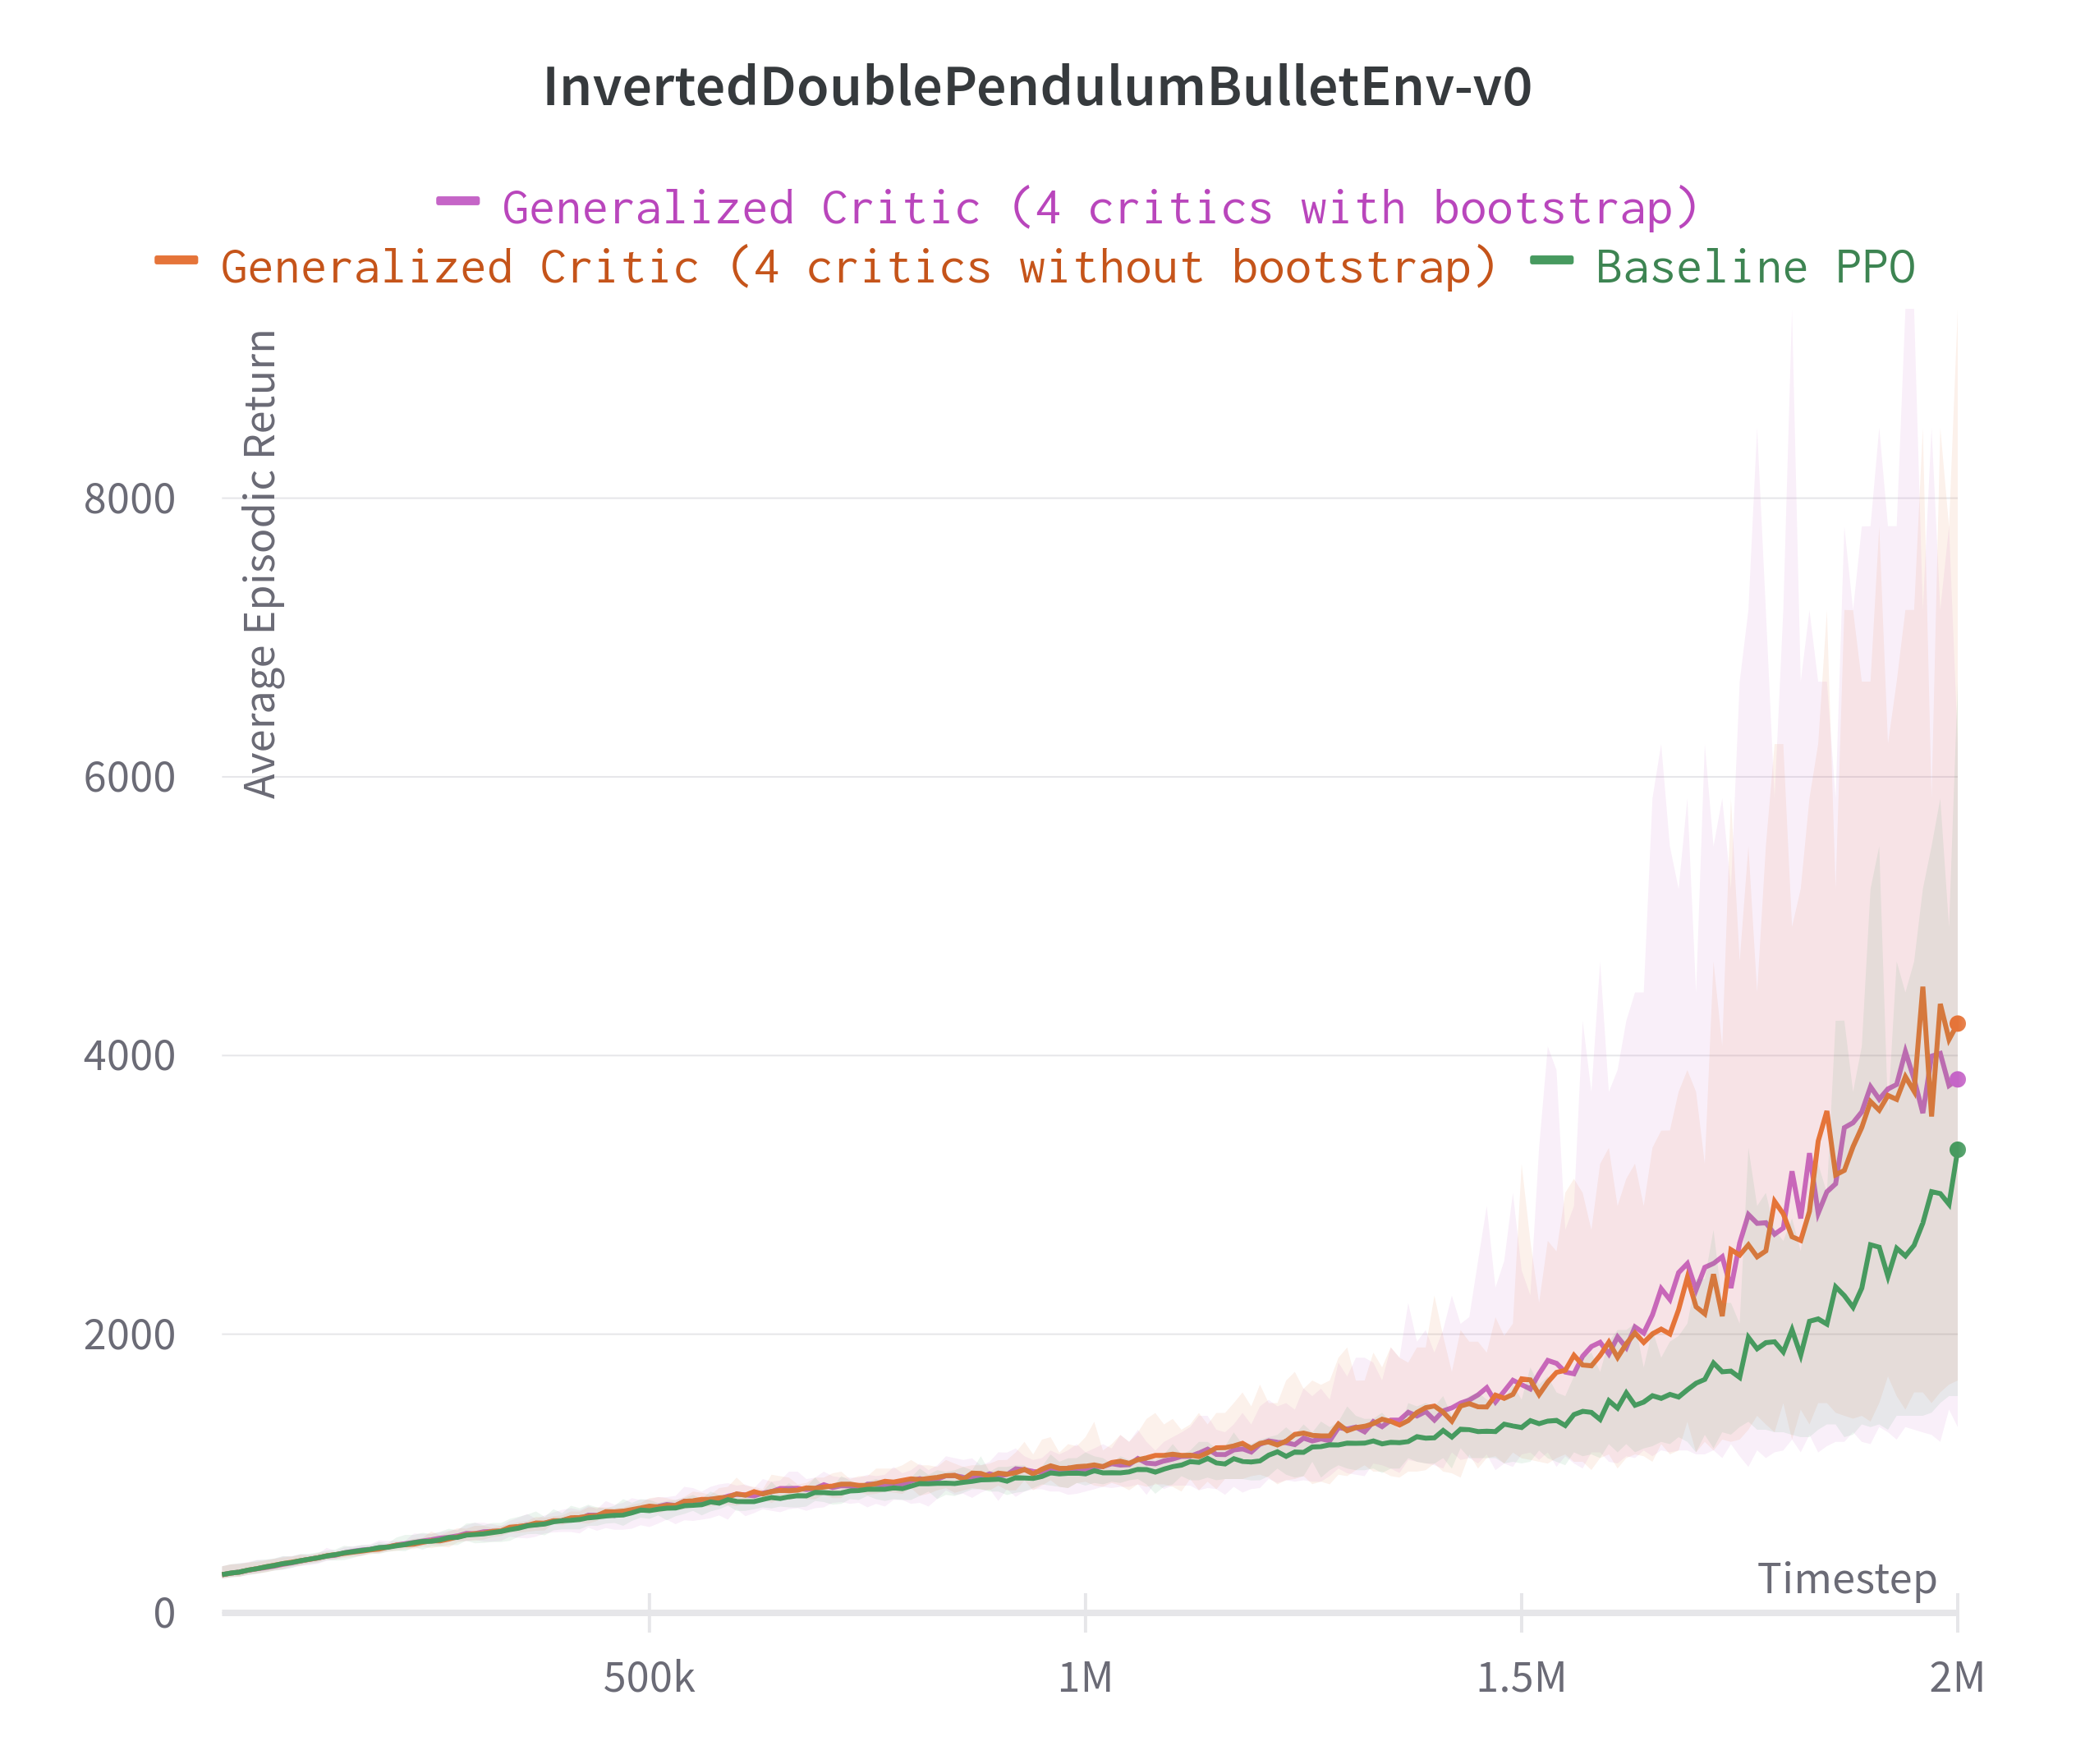
\includegraphics[width=\linewidth]{images/inverteddoublependulum}}
%  \vspace{2.0cm}
%  \centerline{(a) InvertedDoublePendulumBulletEnv-v0}\medskip
\end{minipage}
\begin{minipage}[b]{.5\linewidth}
  \centering
  \centerline{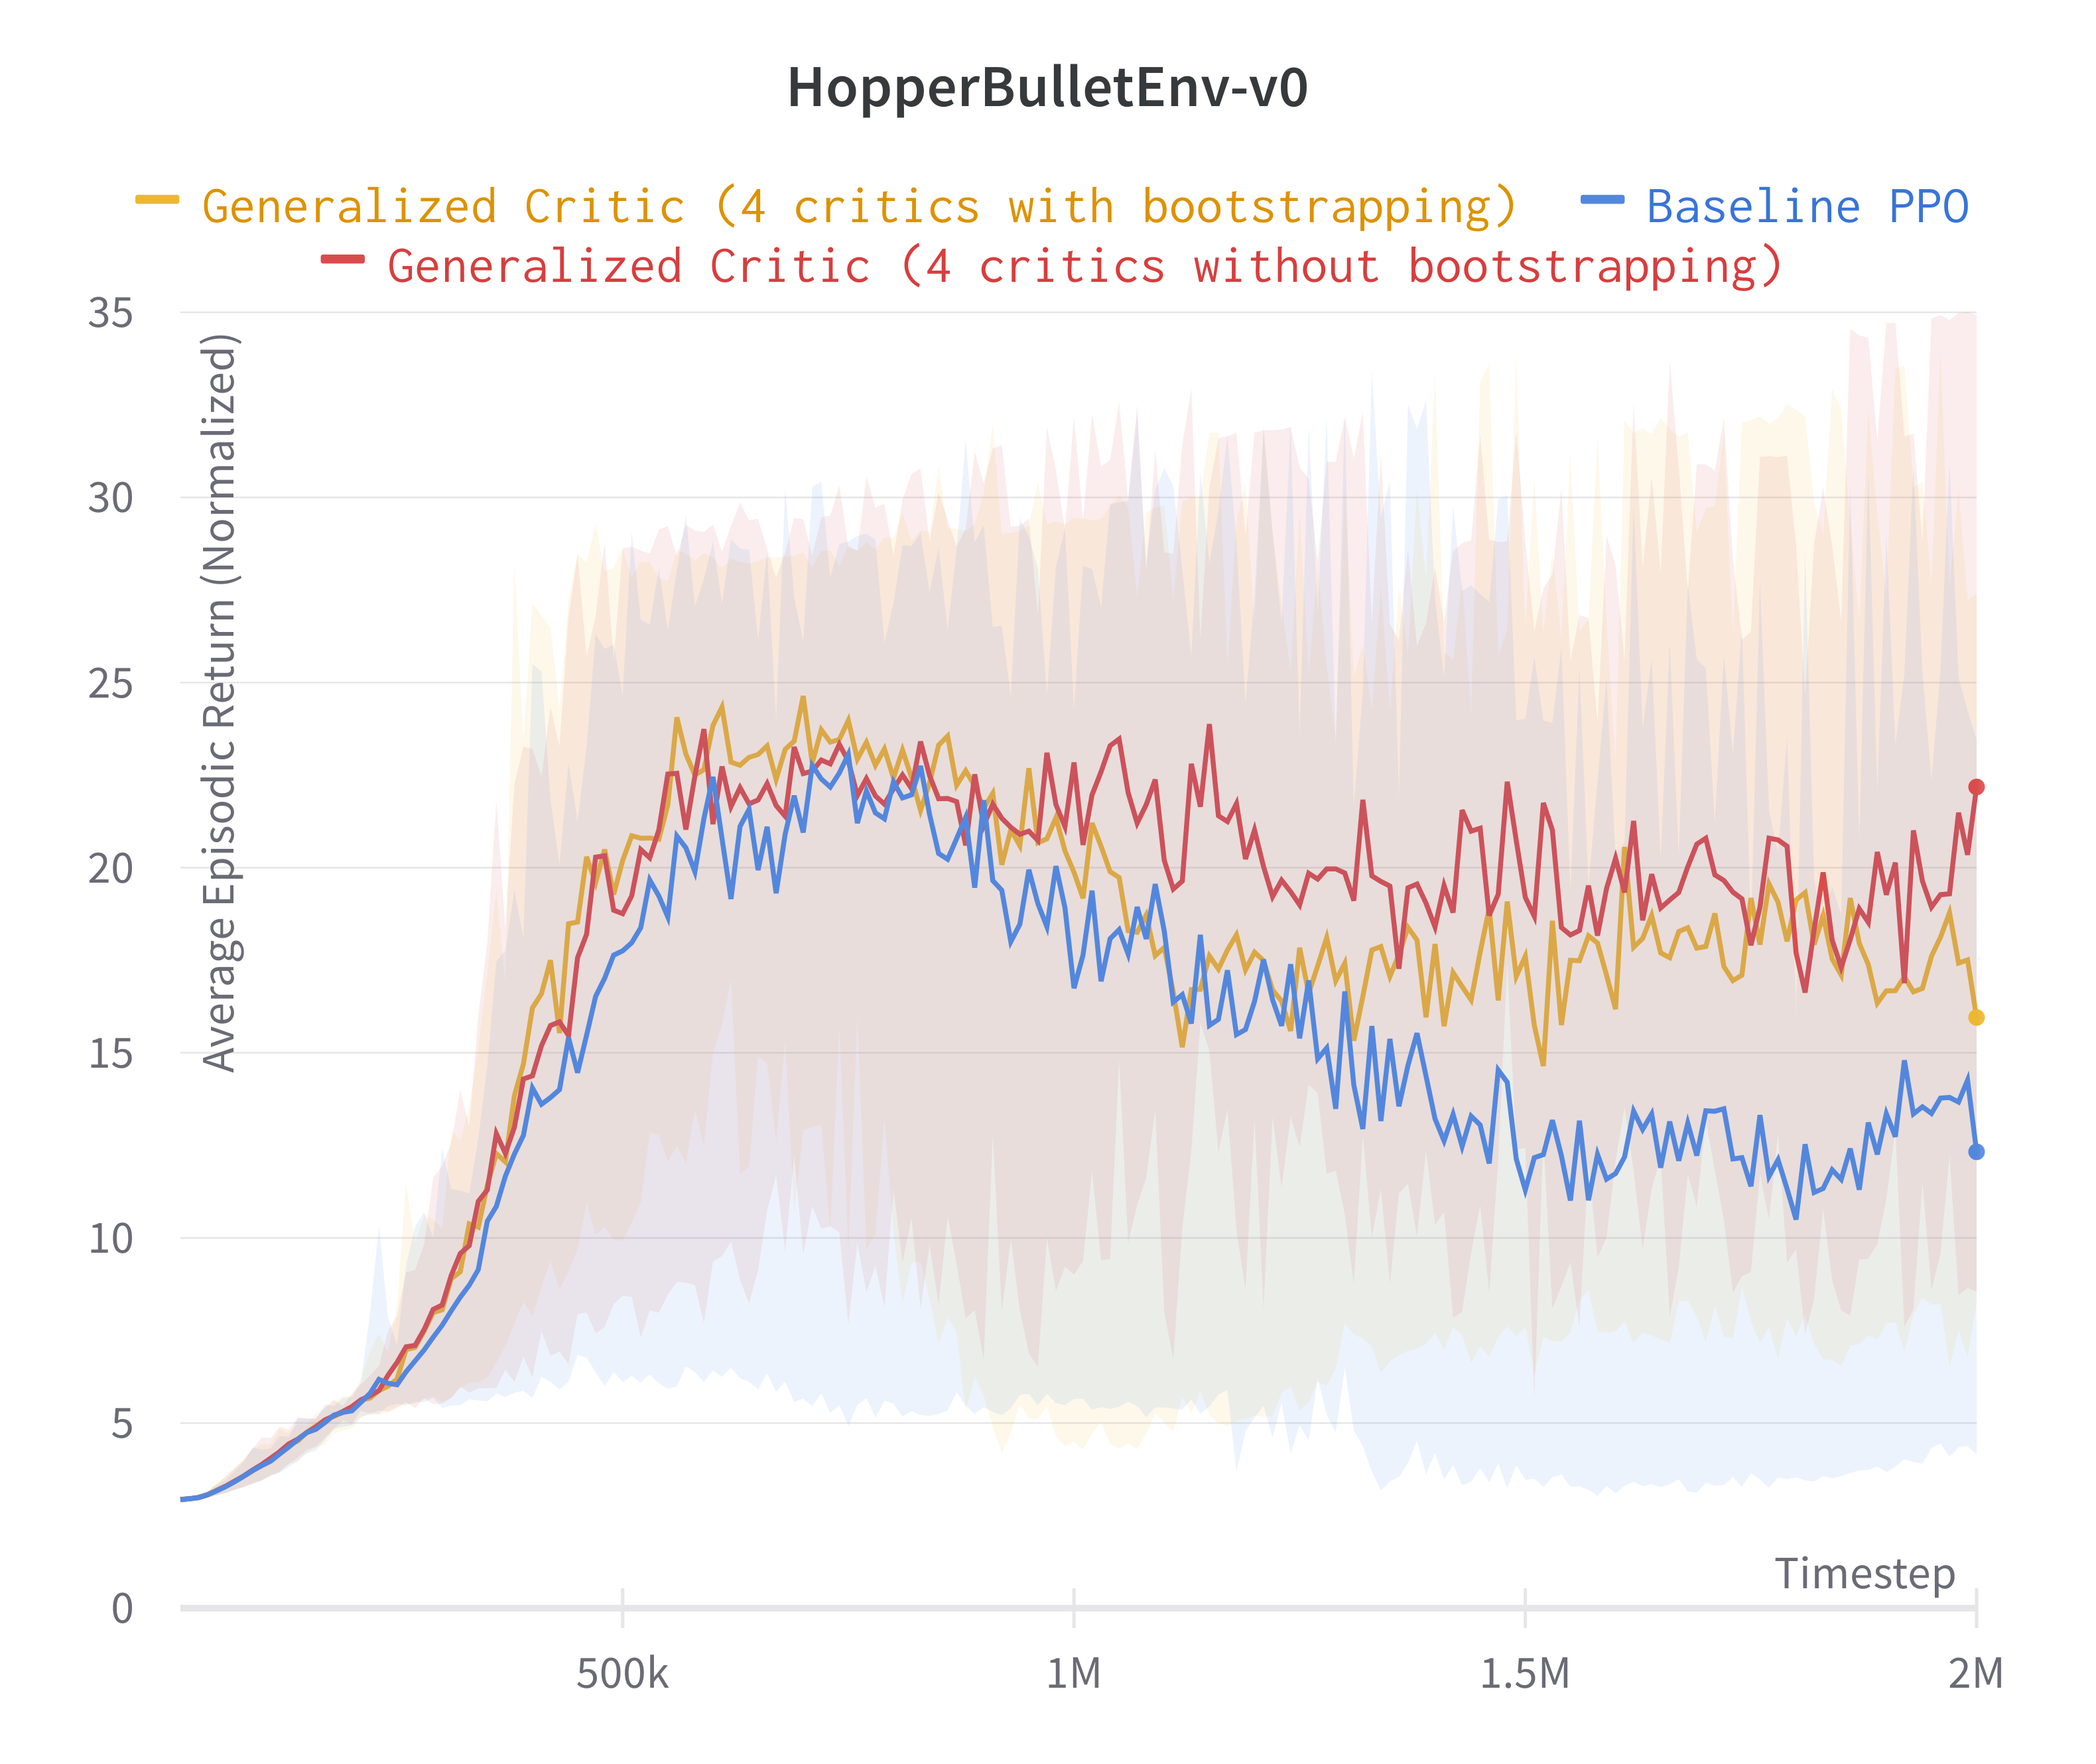
\includegraphics[width=\linewidth]{images/hopper}}
%  \vspace{2.0cm}
%  \centerline{(b) HopperBulletEnv-v0}\medskip
\end{minipage}
\caption{Average performance across 10 random seeds on four environments}
\label{exp2}
\end{figure}
